\cleartooddpage[\thispagestyle{empty}]
\chapter{Analysis}

\section{Studies}
Backgrounds were simplified into radially-symmetric ones.
You can see in these plots ?? how the background changes shape with energy.


\subsection{Effect of Stars}
To examine the effect of stars on the camera, several studies were undertaken.
It had been noted in the past that for a dim star (magnitude > 5??), the given pixel would have a higher average current.
This translated into a higher pedvar??, which can contribute to images, under certain conditions??.

In addition, if a bright star (magnitude <= 5??) was in the field of view, it would cause such a high current in the pixel that it would have to be shut off (voltage set to 0??) to prevent it from being damaged.
For particularly bright stars (magnitude <= 3), often several pixels would be disabled at a given time.

A third effect is that, since the telescope camera is fixed to the ground, from the camera's point of view the sky rotates around the camera center.
This means that over a single 30min observation, any stars rotate around the camera center, disabling several camera pixels as it passes over them.

This implies a key idea, that to study the effect of stars, one should study the effect of high-current or disabled camera pixels, and use this information to construct the effect of stars.

% see calculations/disabledpixel_obstime , those 250 crab runs turned into about 13.5 observation hours
To examine the effects of disable pixels, a study was performed where 13.5 hours of Crab observations were analyzed twice, once normally, and once with a single pixel disabled in all four telescopes.
This mimics the effect of having a star in the field of view that is bright enough to disable a pixel.
Once the events are reconstructed, and passed through gamma-hadron cuts, they can then be compared.
When synchronizing the event lists, it can be done in $O\left(n\right)$ time (rather than $O\left(n^2\right)$ time), as both event lists are already time-ordered.
After the event lists with the pixel enabled and disabled are synchronized, they can be compared.
One can then look for events that disappeared when the pixel was disabled, as well looking for new events that appeared.
Events that are still present in both event lists can then be tested to see how far their reconstructed camera position moved.

In figure \ref{fig:dpix_rel_camera}, the relative event rate in the camera is plotted when pixel 115 is disabled in all four telescopes.
This is calculated by taking, for each bin, the number of reconstructed gamma-like events is divided by the pixel-enabled number of reconstructed events.
It can be seen that there is a loss of events near the disabled pixel (the black circle), with a rate closer to 100\% the further away one goes from the disabled pixel.

\begin{figure}[ht]
  \begin{center}
    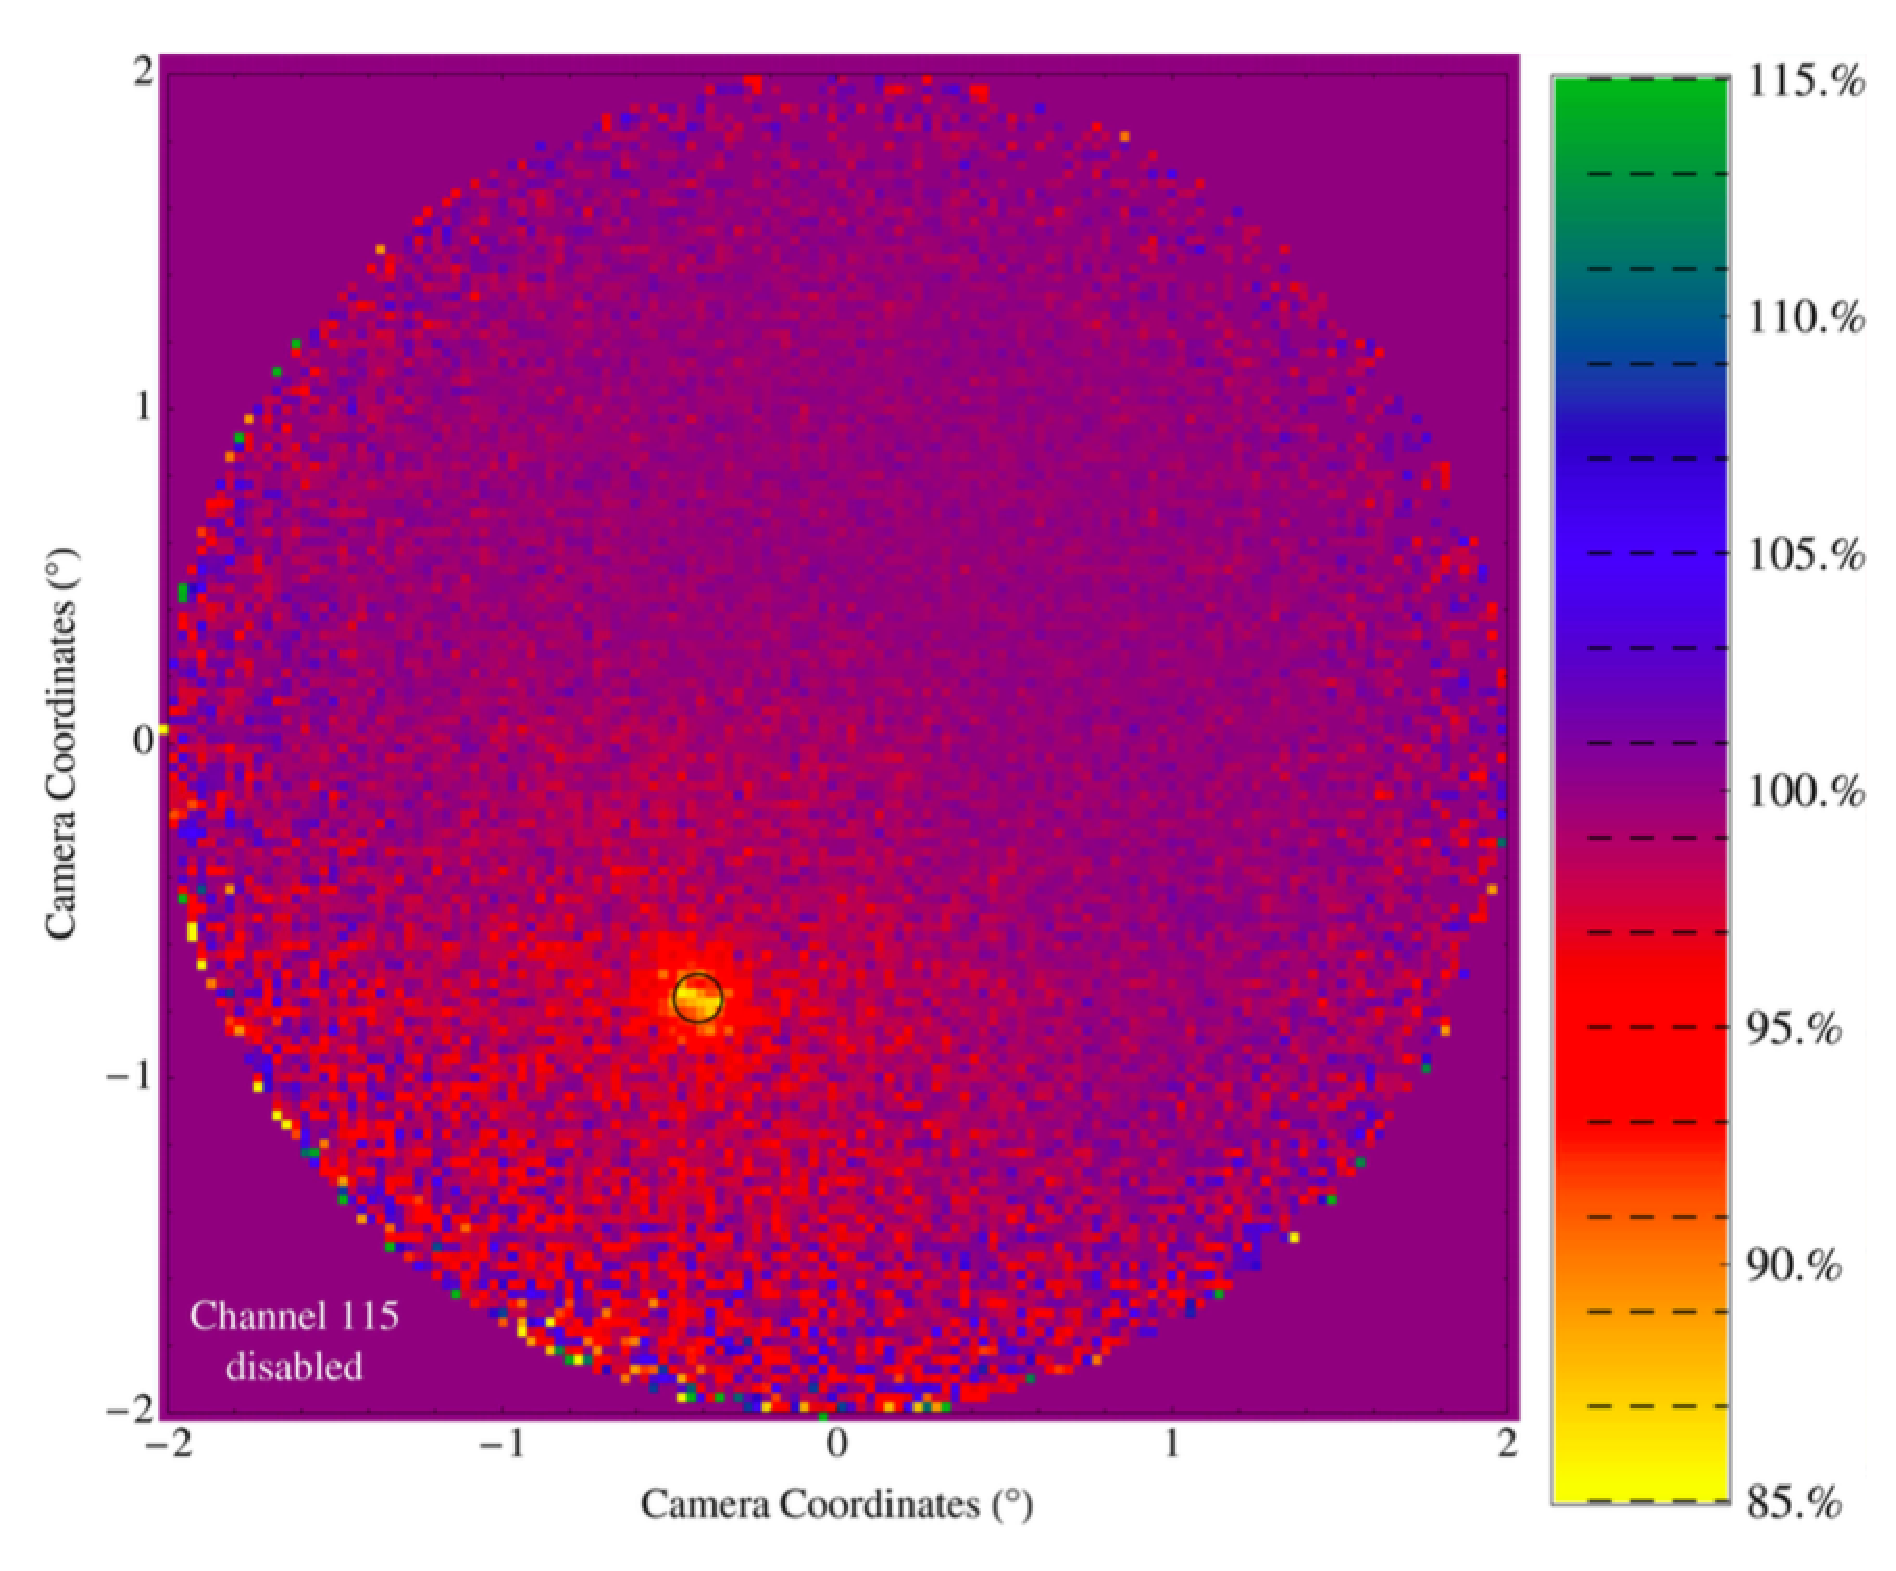
\includegraphics[width=0.8\textwidth]{images/disabled_pixel/relativerate_camera}
    \caption[Relative Event Rate]{Event rate in the camera with pixel 115 disabled (denoted by the black circle) in all four telescopes, relative to having all pixels enabled.  Camera coordinate axes are parallel to azimuth and elevation.}\label{fig:dpix_rel_camera}
  \end{center}
\end{figure}

In figure \ref{fig:dpix_rel_radial}, the bin values from figure \ref{fig:dpix_rel_camera} are divided into radial bins centered around the disabled pixel.
The average relative event rate is then calculated for each bin, along with a 1-sigma distribution width for the error bars.
It can be seen that there are three distinct phases to the plot.
In the first phase, from radius $\ang{0}$ to $\ang{0.3}$, the relative event rate starts extremely low, and rises rapidly.
In the second phase, from radius $\ang{0.3}$ to $\ang{1.6}$, the relative event rate is still rising, but much more slowly.
In the third phase outside $\ang{1.6}$, there is almost no effect.


\begin{figure}[ht]
  \begin{center}
    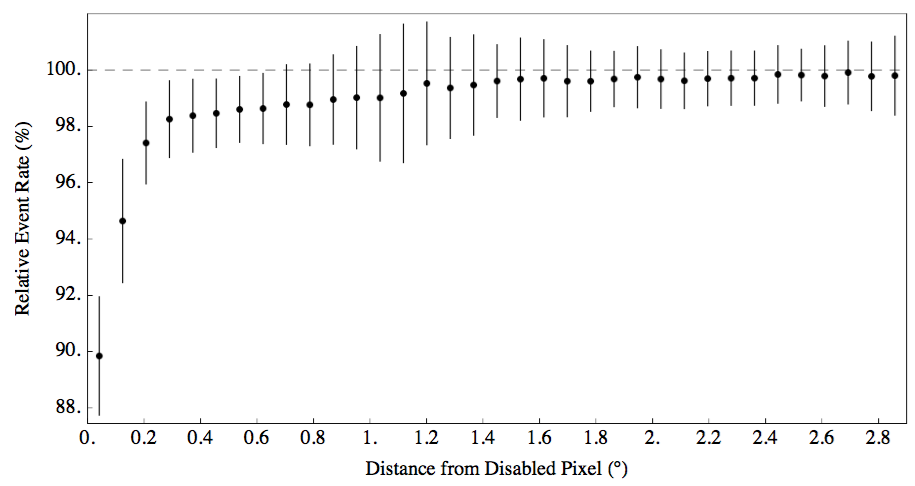
\includegraphics[width=\textwidth]{images/disabled_pixel/relativerate_radial}
    \caption[Radial Relative Event Rate]{Same relative event rate as in figure \ref{fig:dpix_rel_camera}, but averaged into radial bins, centered on the disabled pixel 115. }\label{fig:dpix_rel_radial}
  \end{center}
\end{figure}

In figure \ref{fig:dpix_disappear}, the positions of events that disappeared are shown.
The white area indicates many events are lost in the area of the disabled pixel.
These events would have smaller images, and would be much more susceptable to being cut.

\begin{figure}[ht]
  \begin{center}
    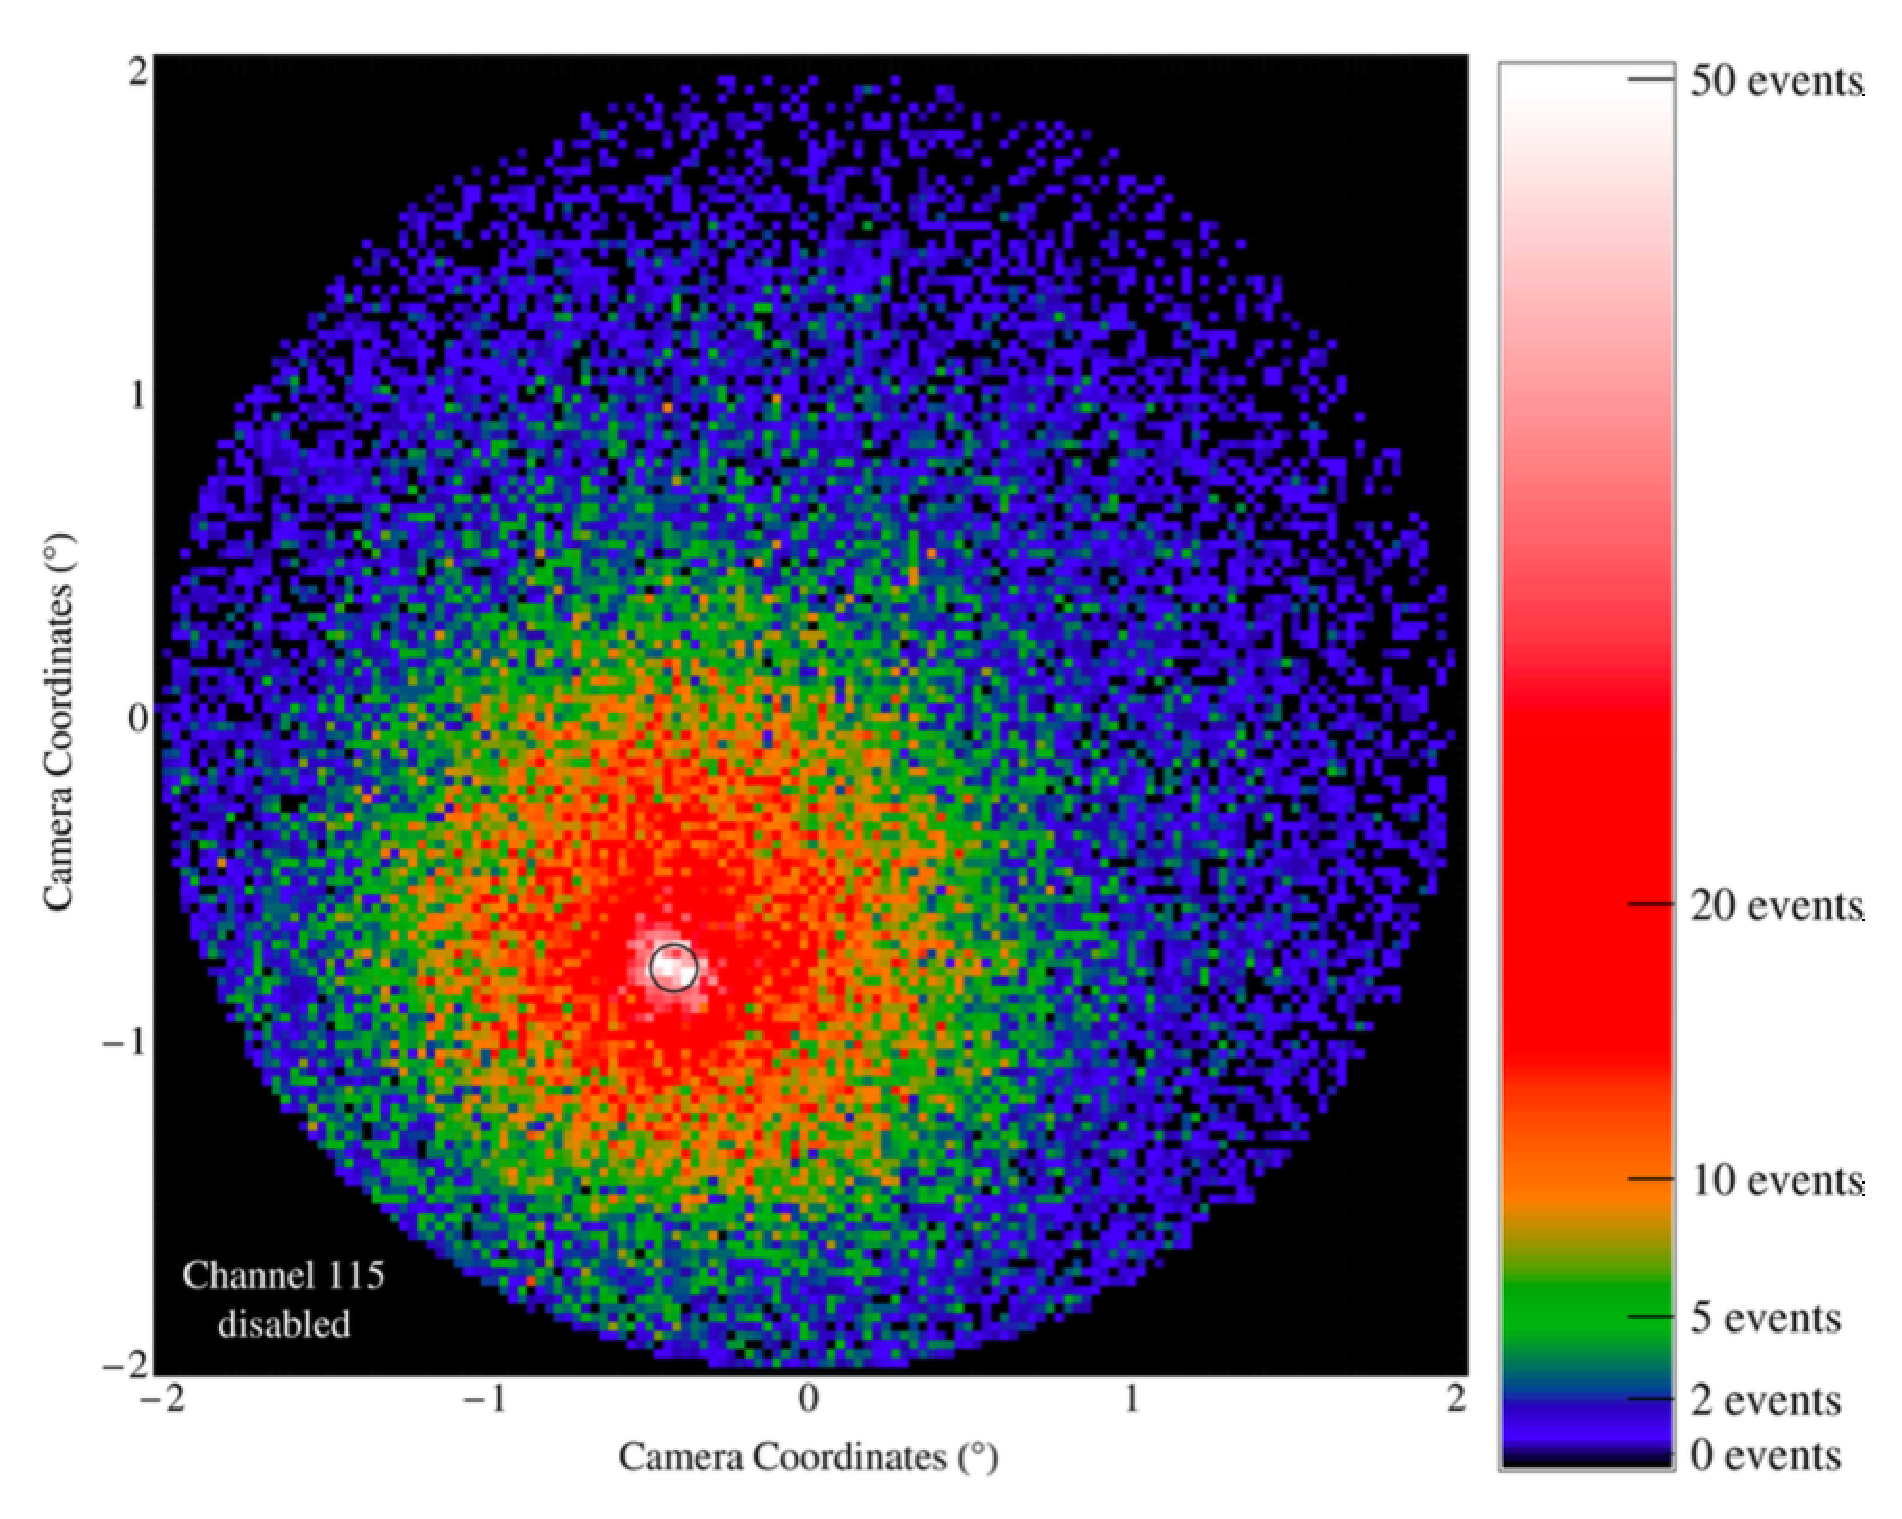
\includegraphics[width=0.8\textwidth]{images/disabled_pixel/disappearing_events}
    \caption[Disappering Events]{Positions of events that disappeared when pixel 115 was disabled in all four telescopes.  Positions are from their pixel-enabled reconstructed position.}\label{fig:dpix_disappear}
  \end{center}
\end{figure}

In figure \ref{fig:dpix_appear}, the positions of events that newly appeared are shown.
It should be noted that these are not events that these are events 'created' by disabling a pixel.
Rather, they are events that, with the pixel enabled, did not pass cuts.
Now that the pixel is disabled, they do pass cuts.

What is also noticeable is that the highest concentration of lost events was in the pixel's area, whereas the highest rate for appearing events is actually in a ring with a radius of \nicetilde1.5 pixels around the disabled pixel.
This is probably due to the fact that disabling a pixel can make some images look thinner or wider, depending on where the disabled pixel is in the image.
A thinner image will look more gamma-like, making it more likely to pass cuts, appearing like 'new' events.
On the other hand, a wider image looks more hadron-like, and is less likely to pass cuts, causing some events to disappear.

\begin{figure}[ht]
  \begin{center}
    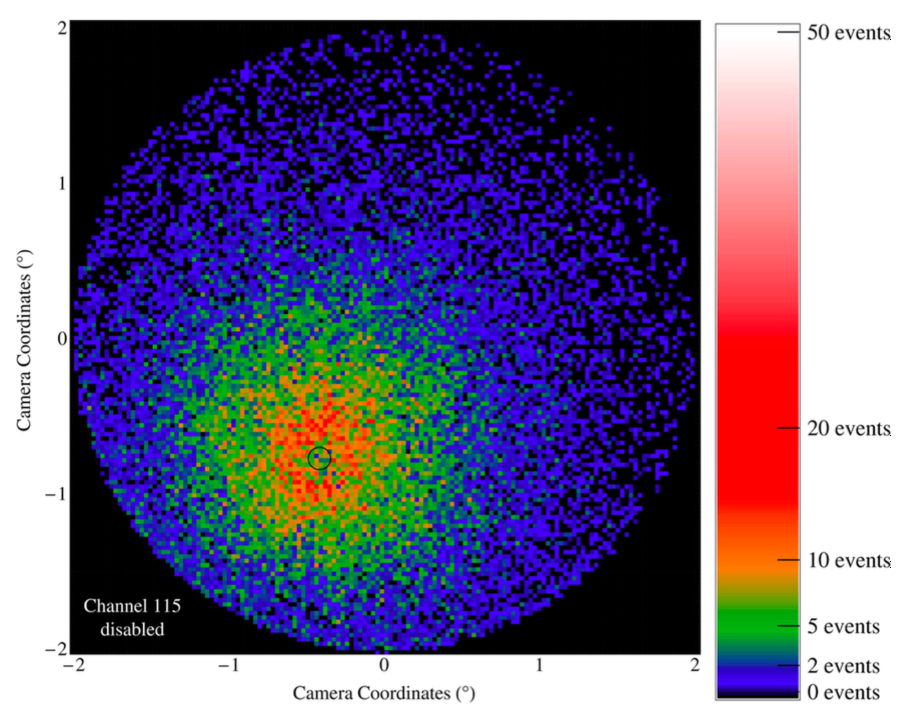
\includegraphics[width=0.8\textwidth]{images/disabled_pixel/appearing_events}
    \caption[Newly Appearing Events]{Positions of new events that appeared when pixel 115 was disabled in all four telescopes.  Positions are from their pixel-disabled reconstructed position.}\label{fig:dpix_appear}
  \end{center}
\end{figure}

In figure \ref{fig:dpix_move}, the movment of gamma-like events is shown, when pixel 115 was disabled in all four telescopes.
Only events which moved more than $0.1*PSF$ are shown.
It should be noted that relatively few (how few??) events move, and the events that do move are mostly ones with strange image shapes that are cut in half when the pixels are disabled.

\begin{figure}[ht]
  \begin{center}
    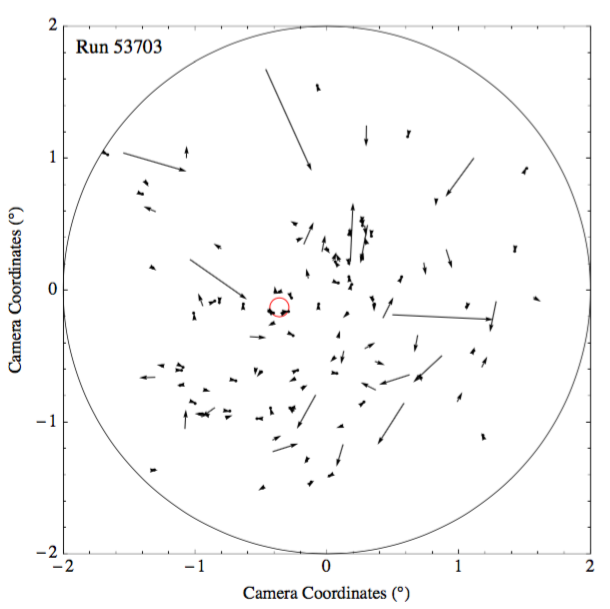
\includegraphics[width=0.8\textwidth]{images/disabled_pixel/moving_events}
    \caption[Event Movement]{Positions of events that moved when pixel 115 (denoted by the red circle) was disabled in all four telescopes.  Arrows point from the pixel-enabled position to the pixel-disabled position.}\label{fig:dpix_move}
  \end{center}
\end{figure}

As the acceptance for a particular event and the event's effective area are strongly related, the loss of acceptance also means a loss of effective area in the area of this pixel.
This can have effects on the energy reconstruction.

For CTA, the pixels are ?? set up so that ?? only one pixel will be shut off at a time due to a bright star.
While this will limit the effect of very bright stars, CTA's planned $\ang{7}$ field of view will mean there are many more stars in view, meaning many more holes to account for.

Future studies could also compare how events move in energy or time when a pixel is disabled.
Another study might investigate how the reconstructed shower-telescope distance changes, since a shower with fewer pixels will look further away, and may be reconstructed differently.
In general, as a pixel is disabled, it is expected that lower energy events and showers further away will be more vulnerable, and will show stronger differences than higher energy events or closer showers.


\subsection{Low Elevations}
For VERITAS, the galactic center is at a low elevation, around $\ang{29}$.
As part of the observing strategy for the galactic center, off data is also taken near the galactic center.
This means that, for most nights when the galactic center is observed (called On runs, at RA/Dec 260.91/-29.01), one 20-30 minute run is also taken with the observatory pointing a few degrees away from the galactic center, at RA/Dec 266.41/-29.01 (called an Off run).
This is done because the galactic center's gamma-ray emissions are highly extended, leaving few regions within the On data that can be used as a background region in the Li and Ma significance equation ??.

At the latitude of the VERITAS observatory, the Galactic Center only rises to a peak elevtaion of $ \nicetilde \ang{30} $, hence, most of the observations are between $\ang{28}$ and $\ang{30}$ elevation.
Almost all other VERITAS observation sources are at elevations higher than $\ang{50}$, so the effects of low elevation observations have not been studied much.
To examine the impact of low telescope elevation on VERITAS observations, several studies were performed.

First, two samples of Galactic Center Off observations were studied, as they had no significant gamma ray sources, and are at very similar elevations to the Galactic Center On observations.
Events from each sample were first divided up into equal-statistics energy bins, to ensure there were enough events in later steps.
Then, for each energy bin, the gamma-like events were binned by their reconstructed position in camera X and Y coordinates.
The Camera X and Y is an angular coordinate system, with the X axis parallel to Azimuth and the Y axis parallel to Elevation, with the origin centered on the telescope pointing target.


In both samples of observations, it can be seen that for the lowest energies, a crescent shape appears, while at the higher energies, the average position of all events is below the center of the camera.


\subsubsection{Higher Elevations}
A similar test was performed with data from higher elevations.
Several other sources were analyzed in a similar manner, to see how strong the effect is, and at what elevation it stops being significant.


\subsection{Diffuse Gamma Rays}

Sets gamma rays were simulated, with corsika, at different energies.
These gamma rays were diffused in a circular disk of radius ?? degrees around ?? elevation/azimuth.
The gamma rays were then processed through the VERITAS simulation chain.
This simulation chain takes the cherenkov photons from each gamma ray shower, and calculates which ones hit telescope mirrors.
Then, it calculates which cherenkov photons hit which pixels, and at what time.
Once cherenkov photons are measured hitting a pixel, a hardware simulation program takes over to simulate the voltage pulse created by the photons.
This voltage pulse is then propagated through a software simulation of the VERITAS triggering system.
Once the list of triggered gamma-ray showers is save to a file, reconstruction of the event can be done by the same software that reconstructs observed events.

\subsection{Elevation Effects}

Diffuse sims with direct-camera pointing show just the elevation effects, no camera effects.
To study the effect of elevation, special diffuse sims were made.
These were produced such that, after creating diffuse gamma rays in corsika, the simulated telescopes were pointed directly at each event.
This means that while the events were at a variety of azimuths and elevations, they all hit in the center of the camera.

From these plots, one can see that different gamma-ray energies have different horizon elevations, below which a particular energy gamma ray cannot be detected.

By looking at the number of gamma rays detected at each energy and elevation (and ignoring azimuth), the slope of the elevation effect can be seen.
It is important to note, that each energy has a different slope due to elevation.


\subsection{Gamma Verses Protons}

Doughnut shapes appear in the gamma-like protons.


\section{Veritas Data}
runs/sources/dates/times

\section{Likelihood Ratio Test}
The likelihood ratio test useful for comparing two hypotheses.
They are referred to as the null and alternative hypotheses.
Each hypothesis consists of a predicted number of events at each point in the energy/space/time parameter space.
Once each hypothesis is constructed, the likelihood for each can be computed.
The ratio of the two likelihoods then follows a gaussian (with certain assumptions), meaning the sigificance of the alternative hypothesis over the null can be calculated.

\section{Backgrounds}

Backgrounds estimate the amount background events in the camera.
For the past several years, the backgrounds used in Event Display only depended on the distance between each event's reconstructed position and the center of the camera.
From the studies in section ?? it was found that at low elevations, there is also dependence on the event's position around the camera center (camera $\phi$ angle), as well as the events energy.
As a consequence of the $\phi$-angle dependence, this also means the background is time-dependent as well, on the order of minutes.
Accounting for this in Event Display code would have taken much longer than the available time, so for this analysis, the simple $\phi$-symmetric backgrounds were used.

Backgrounds were made from several hours of Galactic Center Off runs.
These runs were pointing ?? degrees from the camera center, to avoid effects of the disk, and to help account for the higher noise and any elevation effects.

\section{Test Crab Analysis}

Only studied runs with elevations between $\ang{70}$ and $\ang{75}$.
Used Segue 1 data at the same elevations as a background.

\subsection{Event Display}
\subsection{CTOOLs}

\section{Sgr A* Data Analysis}
Broke data into two elevation regimes, $ \ang{25}-\ang{28.5} $, and $ \ang{28.5}-\ang{30.25} $.
Separate off runs were taken to use as a background.

  \subsubsection{Event Display}

\section{Astrophysical Models}

\subsection{Point Sources}

\subsection{Diffuse Emission}

\subsection{Dark Matter}
Dark Matter halos are modeled by a spherically-symmetric mass-per-volume density profile.
Two promising candidates for this profile are Einasto and Navarro-Frenk-White (NFW) profile.

The Einasto profile takes the form:
$ \rho\(r\) = \rho_{o} exp \{ - \frac{2}{\alpha} \[ \(\frac{r}{r_o}\)^{\alpha} - 1 \] \} $
(This is from http://journals.aps.org/prd/pdf/10.1103/PhysRevD.83.023518 , check it against other source's definitions of the Einasto profile??)

(Plot of density profiles??)

(Plot of J-factors??)


\section{Upper Limit}

comparison to 

